\section{Planning and Learning with Tabular Methods}
\subsection{Exercise 8.1}
\subsubsection{Q}
The nonplanning method looks particularly poor in Figure 8.3 because it is a one-step method; a method using multi-step bootstrapping would do better. Do you think one of the multi-step bootstrapping methods from Chapter 7 could do as well as the Dyna method? Explain why or why not.
\subsubsection{A}
If we used a multi-step bootstrapping method (e.g. n-step Sarsa), we could back-propogate the reward from the final timestep along the trajectory followed for some large value of $n$. This of course would only update the action-values of the $n$ action-values prior to receiving the reward and leave the remain 1700 - $n$ action values unchanged. When running a second episode using this approach, the agent would still act naively until it reached its first state-action pair with some value, which it could then bootstrap from to update previous states. Without a model of the environment (like Dyna) it cannot plan in the same way, and cannot reap the efficiency gains that Dyna enjoys. 

$
\hfill \blacksquare
$

\subsection{Exercise 8.2}
\subsubsection{Q}
Why did the Dyna agent with exploration bonus, Dyna-Q+, perform better in the first phase as well as in the second phase of the blocking and shortcut experiments?
\subsubsection{A}
I'm not sure it is performing \textit{better}, rather that the Dyna-Q+ algorithm is increasing the reward associated with every state at every timestep when Dyna-Q is not, so cumulative reward must be higher in absolute terms than Dyna-Q. In this sense a direct comparison on the basis of cumulative reward is perhaps unfair. Due to the increased exploration of the Dyna-Q+ algorithm, it is however likely that it found the optimal policy more quickly than Dyna-Q and so was able to exploit it quicker for higher cumulative reward

$
\hfill \blacksquare
$

\subsection{Exercise 8.3}
\subsubsection{Q}
Careful inspection of Figure 8.5 reveals that the difference between Dyna-Q+ and Dyna-Q narrowed slightly over the first part of the experiment. What is the reason for this?
\subsubsection{A}
Dyna-Q+ is forced to explore continually having already obtained the optimal policy, meaning that when Dyna-Q is exploiting its learned optimal policy, Dyna-Q+ is exploring sub-optimal trajectories and receiving less reward.

$
\hfill \blacksquare
$

\subsection{Exercise 8.4}
\subsubsection{Q}
The exploration bonus described above actually changes the estimated values of states and actions. Is this necessary? Suppose the bonus $k\sqrt{\tau}$ was used not in updates, but solely in action selection. That is, suppose the action selected was always that for which $Q(S_t, a) + k\sqrt{\tau(S_t, a)}$ was maximal. Carry out a gridworld experiment that tests and illustrates the strengths and weaknesses of this alternate approach.
\subsubsection{A}
\ProgrammingExercise \\
\begin{figure}[h!]
	\centering
	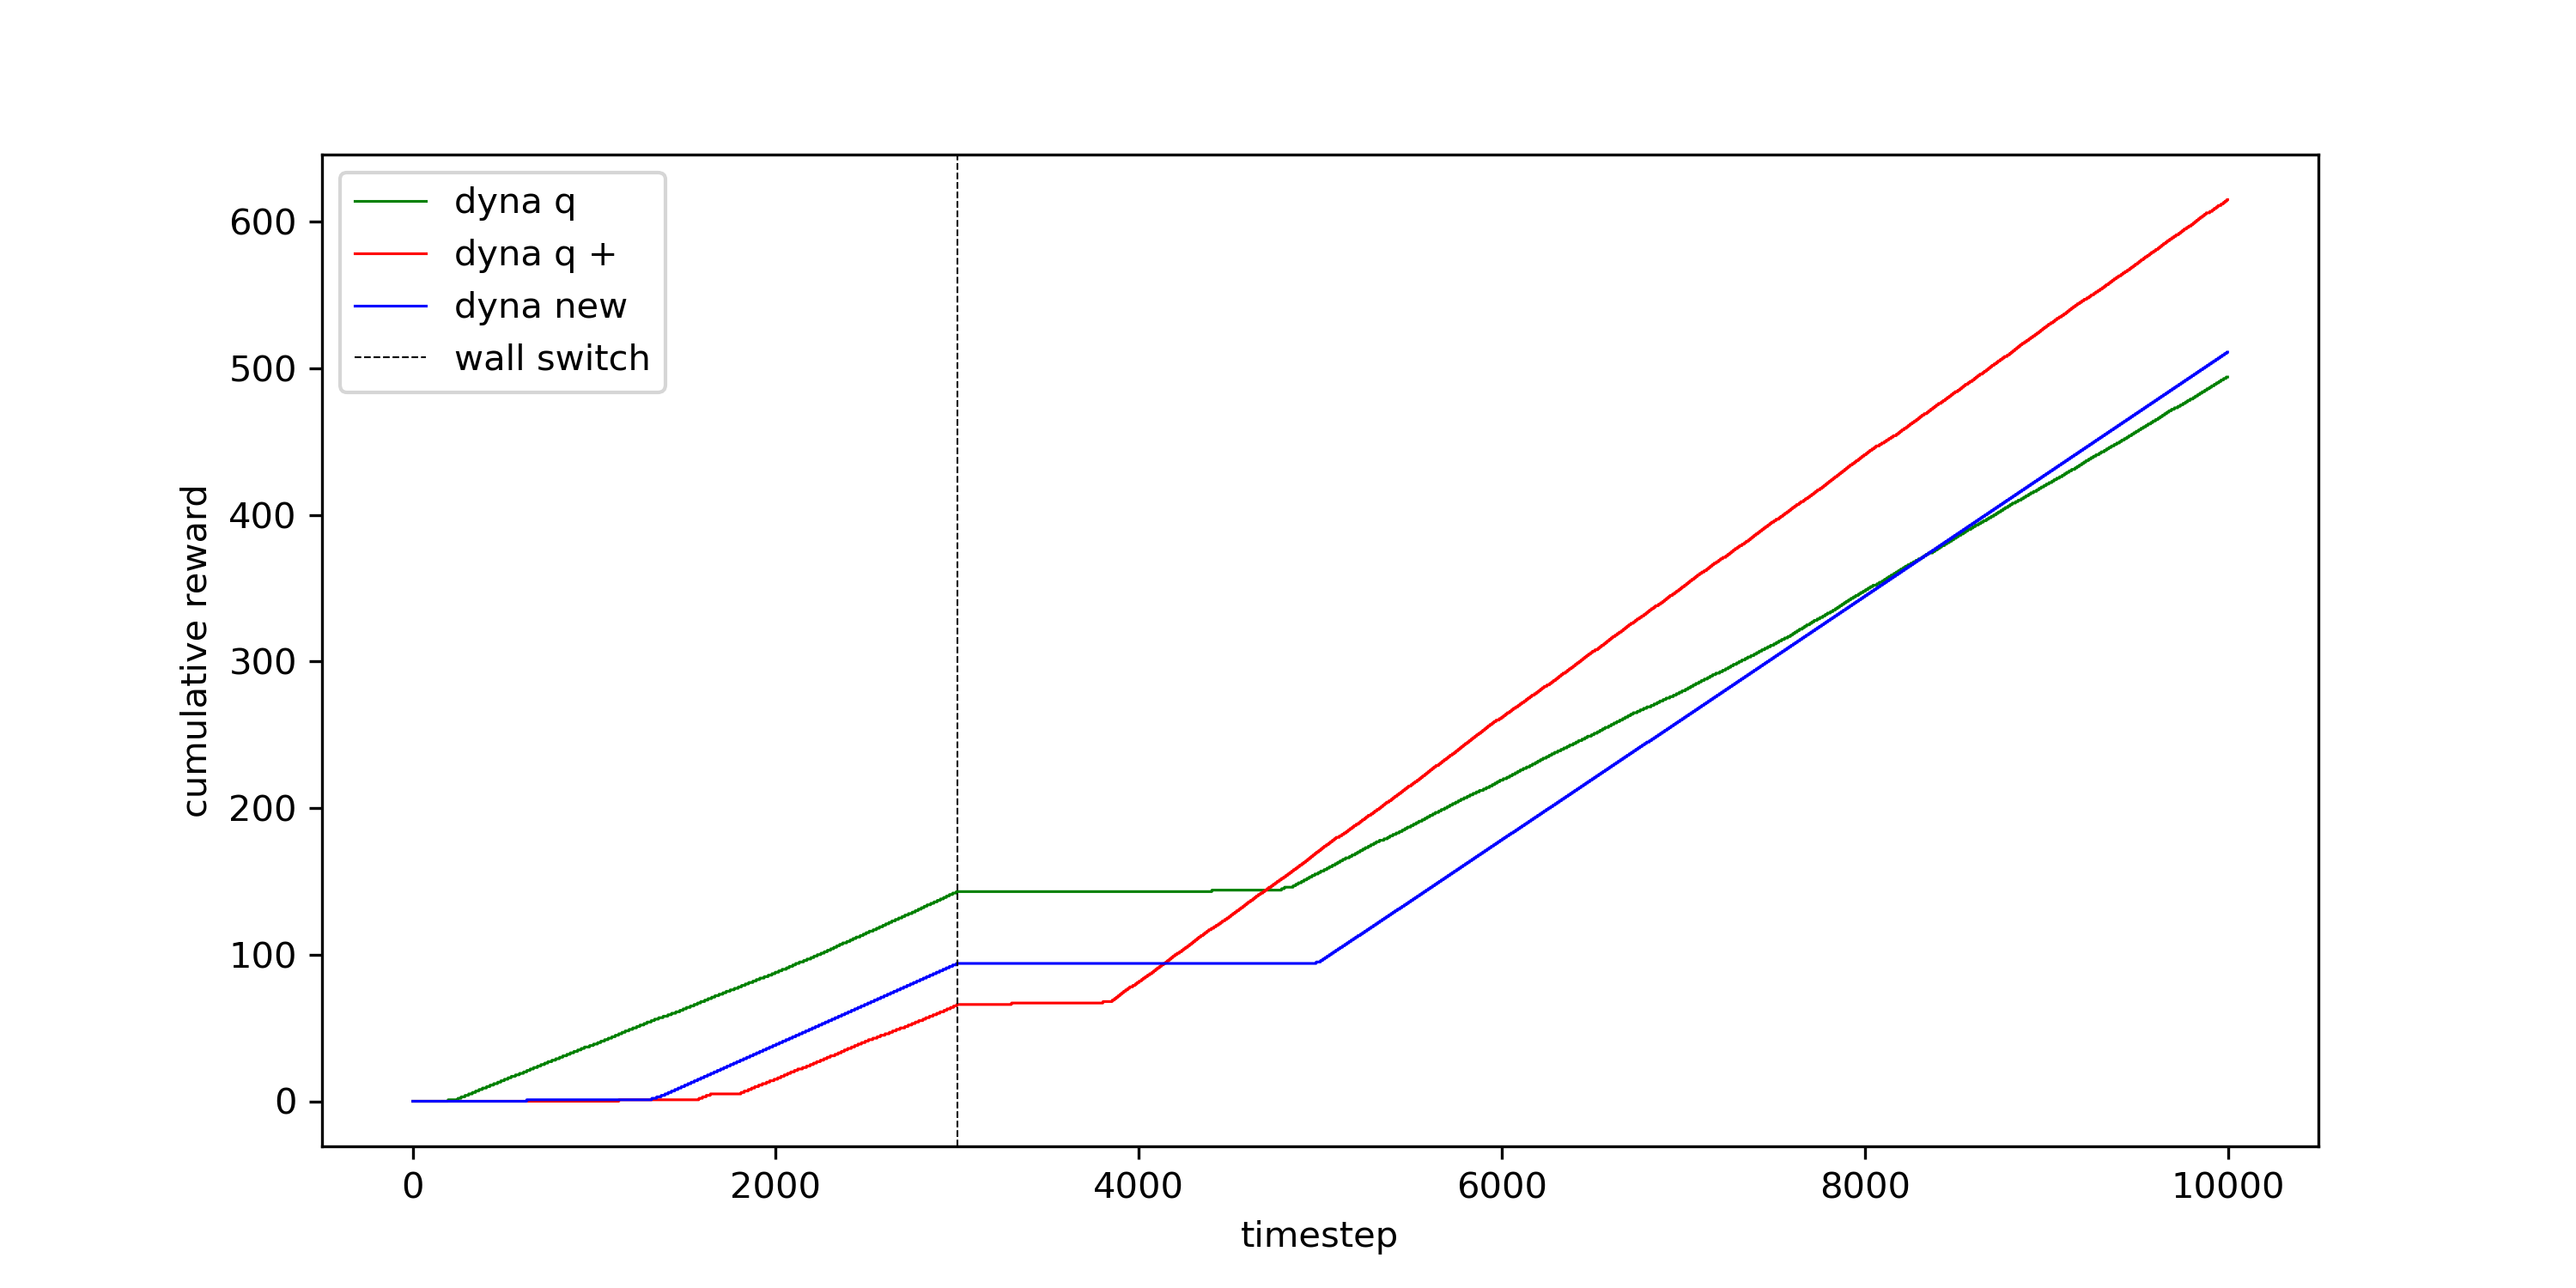
\includegraphics[width=\textwidth]{/ex8.4}
	\caption{Cumulative reward for three model-based agents on the blocked maze task after 10000 timesteps}
	\label{fig: 8.4}
\end{figure}
Summary of the models:
\begin{description}
\item[Dyna Q] uses a conventional $e$-greedy policy, and plans with a model that uses only previously received states and rewards. 
\item[Dyna Q+] uses a conventional $e$-greedy policy, and plans with a model that gives additional value to the action proportionate to the time passed since they were last selected. Doing so adds arbitrary value to the value function.
\item[Dyna New] uses a novel policy that adds value to each action before selection, in the same way as Dyna Q+, then selects the value maximising action. This combines exploration and exploitation unlike the above two that keep these regimes separate.
\end{description}

Figure \ref{fig: 8.4} illustrates the different learning rates of the three agents. Dyna Q learns fastest initially as it can use its model to learn the optimal policy quickly, but struggles to adapt to the maze block changes after timestep 10000 as its model is inflexible to change. Dyna Q+ has a higher degree of exploration than Dyna Q (because it explores both in the real environment and the simulated environment while planning) and so does not find the optimal policy as quickly as Dyna Q. It does, however, adapt to the wall switch speedily, and exploits its new knowledge to find the optimal policy. Finally, Dyna New, finds the optimal policy before the wall switch, then struggles to capture it post-switch. This is because Dyna New cannot perform exploration in planning, it only explores when taking actions in the real environment. This means that it will take many timesteps before a string of actions taking it to the other side of the grid build enough value for it to be explored. 

Dyna Q Plus performs best in the long run by combining exploration in planning, and exploitation in the real environment. It does however seem these results are subject to initialisation and hyper-parameters. In some runs of the experiment Dyna New never found the optimal policy before the wall switch, its performance seems to be closely linked to the initialisation of $\tau$

$
\hfill \blacksquare
$

\subsection{Exercise 8.5}
\subsubsection{Q}
How might the tabular Dyna-Q algorithm shown on page 164 be modified to handle stochastic environments? How might this modification perform poorly on changing environments such as considered in this section? How could the algorithm be modified to handle stochastic environments \textit{and} changing environments?
\subsubsection{A}
\begin{figure}[h!]
	\centering
	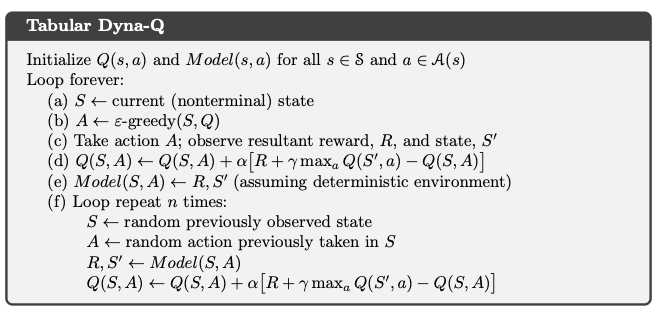
\includegraphics[width=\textwidth]{/ex8.5}
	\caption{Tabular Dyna-Q algorithm}
	\label{fig: dyna-Q}
\end{figure}
\begin{itemize}
\item In part (e) of the algorithm, instead of updating $R$ and $S'$ directly, we would store samples of $R$ and $S'$ from which we can compute distributions and thus expectations. 
\item This would perform poorly because it would be bias toward earlier observations made in the unchanged environment.
\item We could likely rectify this by weighting more recent observations, or discounting past observations in the distribution. Equally we could quantify the agent's confidence in its model e.g. if it hasn't selected a state-action pair in a long time, its confidence in its model should be low and vice versa. This could manifest as a relationship with $\tau$ as discussed with Dyna-Q+.
\end{itemize}

$
\hfill \blacksquare
$

\subsection{Exercise 8.6}
\subsubsection{Q}
The analysis above assumed that all of the $b$ possible next states were equally likely to occur. Suppose instead that the distribution was highly skewed, that some of the b states were much more likely to occur than most. Would this strengthen or weaken the case for sample updates over expected updates? Support your answer. 
\subsubsection{A}
A skewed distribution would strengthen the case for sample-based updates. We are more likely to sample from weighted parts of the distribution and so our estimate of the expected value will approach the true value quicker than would be the case with a uniform distribution i.e. our initial samples will provide a good estimate of the true value. The expectation will require the same computational effort regardless of the shape of the distribution.

$
\hfill \blacksquare
$

\subsection{Exercise 8.7}
\subsubsection{Q}
Some of the graphs in Figure 8.8 seem to be scalloped in their early portions, particularly the upper graph for b = 1 and the uniform distribution. Why do you think this is? What aspects of the data shown support your hypothesis?
\subsubsection{A}
In the uniform distribution case with $b=1$ the start-state is updated every $|\mathcal{T}|$ updates, at which point it's value will be moved toward it's new value.  Whereas in the on-policy case, the start state is visited with probability $0.1$ (given this is the probability of termination)  and so it is updated far more regularly. The time taken to wait for the updates in the uniform case (when other states not close to the start state are being updated) is when the scallops appear in the curves. 

$
\hfill \blacksquare
$